\section{The Standard Model- A Brief Overview}
The Standard Model of particle physics which has been one of the most successful and well-tested theories so far, provides the most fundamental description of nature by incorporating the elementary particles and their interactions. These elementary particles are categorized into two families: fermions (having half integer spins) which form matter as we know it, and bosons (with integer spins) serving as mediators of the three fundamental forces. While electromagnetic interactions are mediated by the photon ($\gamma$); strong and weak interactions are mediated by gluons (g) and by $W^{\pm}, Z^{0}$ bosons respectively. A fundamental particle that mediates gravitation has been only postulated theoretically, and is left out of the Standard Model, since the effects of gravity are too weak to play any important role in the realm of particle physics. 

\begin{figure}[h!]
\centering
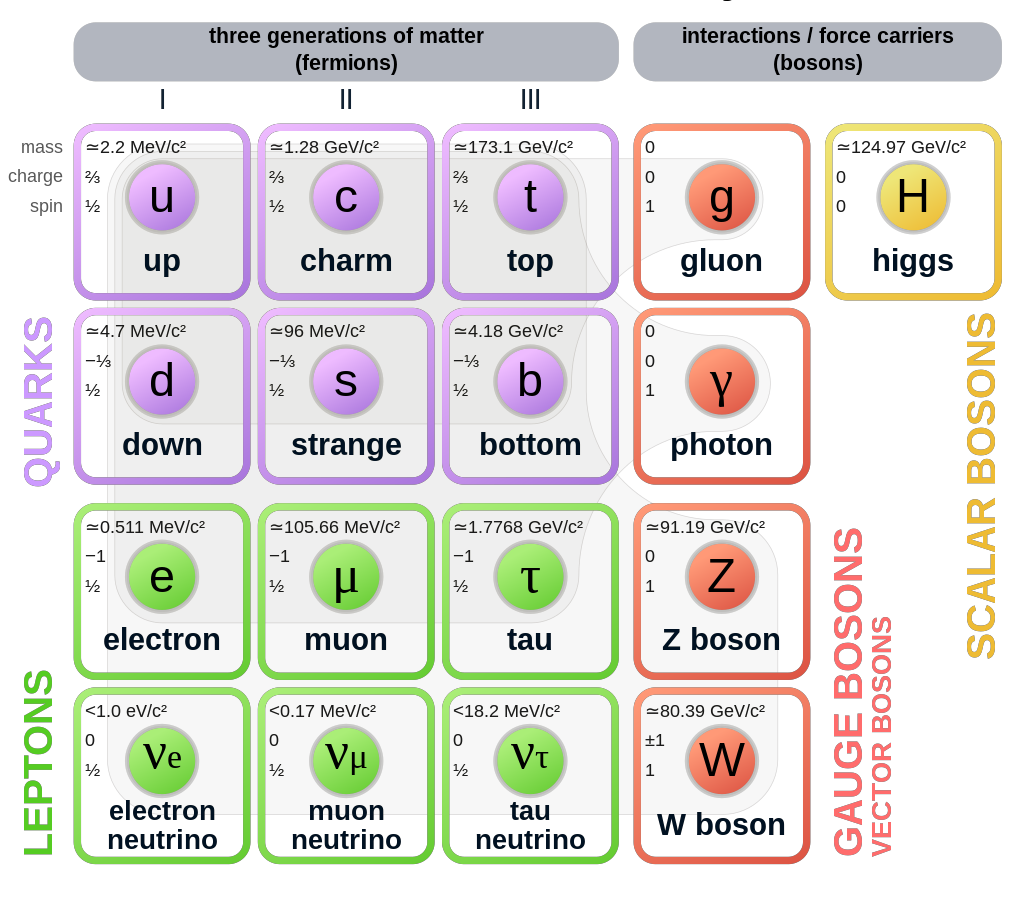
\includegraphics[scale=0.4]{./images/Standard_Model_of_Elementary_Particles.png}
\caption[The Standard Model of elementary particles]{A chart showing the families of elementary particles in the Standard Model \cite{stdmodel}}
\label{fig:StdModel}
\end{figure}

The fermions consists of three generations of quarks and leptons. The quarks have six flavours: up (u), down (d), charm (c), strange (s), top (t) and bottom (b). Similarly, the leptons consist of the electron ($e$), muon ($\mu$) and tau ($\tau$), each having its own associated charge-less and almost massless neutrino ($\nu_{e}$, $\nu_{\mu}$ and $\nu_{\tau}$). Furthermore, each particle in the standard model has its own antiparticle. The quarks are able to form composite particles in either three quark combinations, called baryons ($qqq$/$\bar{q}\bar{q}\bar{q}$) or a quark-antiquark pair, called a meson ($q\bar{q}$). Mathematically, the elementary particles are described as elements of representations of certain symmetry groups. The gauge fields that couple to these particles (i.e. mediate the interactions) arise naturally as a consequence of invariance of their corresponding Lagrangian under local group transformations \cite{thomson_2013}. As such, the gauge symmetry that governs the Standard Model is given by: $$SU(3)_{\mathrm{Colour}}\times SU(2)_{\mathrm{Left\ chiral}}\times U(1)_{\mathrm{Y}(\mathrm{Weak \ hypercharge})}$$

\section{The Unified Theory of Electromagnetic and Weak Interactions}
Since the experiment deals with verifying some of the properties of the $Z^{0}$ bosons, it is of interest to touch upon the theory of electroweak unification.

While electromagnetism and the theory of weak interactions were formulated separately, it was later on postulated that at higher energies ($\sim$ 246 GeV \cite{pdg-ew}), both these interactions would be unified into a single force. As such, the GSW(Glashow-Salam-Weinberg) electroweak model was developed in the 1960s to describe this unified force. 

One finds that imposing the principle of local gauge invariance on the $SU(2)_{L}$ symmetry group leads to the introduction of three gauge fields: $W^{(1)},\ W^{(2)}$ and $W^{(3)}$ (or $W^{0}$ in some references) \cite{thomson_2013}. The physical $W^{+}$ and $W^{-}$ bosons (that mediate the weak charged current interaction) can be seen as the linear combinations: 
\begin{equation}
W^{\pm}=\dfrac{1}{\sqrt{2}}\left(W^{(1)}\mp W^{(2)}\right)
\end{equation}
However, the $W^{(3)}$ field has no physical interpretation of its own. Therefore an additional symmetry, the $U(1)_{Y}$ group is introduced. The field $B$ (or equivalently $Y^{0}$) arising as a consequence of this new symmetry, similarly does not have a physical meaning on its own. Rather, it was seen that linear combinations of the $W^{(3)}$ ($W^{0}$) and $B$ ($Y^{0}$) fields gives rise to the  photon and the $Z^{0}$ boson:

\begin{equation}
\begin{pmatrix} 
\gamma \\ 
Z^{0} 
\end{pmatrix}
= 
\begin{pmatrix}
\cos \theta_{W} & \sin \theta_{W} \\
-\sin \theta_{W} & \cos \theta_{W} 
\end{pmatrix}
\begin{pmatrix}
B \\
W^{(3)}
\end{pmatrix}
\end{equation}
where $\theta_{W}$ is the weak mixing/Weinberg angle

In addition to this, it is to be noted that the gauge fields $W^{(1),(2),(3)}$ and $B$ have to be massless, in order to respect gauge invariance under local $SU(2)_{L}\times U(1)_{Y}$ gauge transformation. However, the physical gauge bosons $W^{\pm}$ and $Z^{0}$ are predicted to be massive, whereas the photon should remain massless. To explain this, the concept of electroweak spontaneous symmetry breaking was introduced. A massive scalar field (the Higgs field) is introduced, to which these bosons ($W^{\pm}$, $Z^{0}$) must couple to, in order to get their physical masses, while the photon does not interact with it \cite{Dooling:207610}. The intricacies of the Higgs mechanism are not of immediate interest here, and can be understood from standard references \cite{thomson_2013, Griffiths:111880}.

\section{Physics Related to the $Z^{0}$ Resonance}
\subsection{$e^{+}e^{-}$ Interactions}
Before discussing the processes of interest involving $Z^{0}$ production, we first list out the important ways in which $e^{+}e^{-}$ pairs can interact \cite{UB}:
\begin{itemize}
\item $\bm{e^{+}e^{-}\rightarrow e^{+}e^{-}}$: Bhaba scattering (elastic scattering) of $e^{+}e^{-}$ pairs 
\item $\bm{e^{+}e^{-}\rightarrow e^{+}e^{-}\gamma \gamma}$: two photon process; $e^{+}e^{-}$ can scatter off of virtual photons, arising out of the incoming $e^{-}$ and $e^{+}$ themselves and these photons can then produce hadrons
\item $\bm{e^{+}e^{-}\rightarrow f \bar{f}}$: Electron-positron pairs annihilate to produce a gauge boson ($\gamma$ or $Z^{0}$), which would in turn produce a fermion-antifermion ($f\bar{f}$) pair. Here $f\bar{f}$ are fermions other than $e^{+}e^{-}$ since that process is already included under Bhaba scattering.
\item $\bm{e^{+}e^{-}\rightarrow \gamma \gamma / \gamma \gamma \gamma}$: An electron-positron pair could also produce two or three photons 

These $e^{+}e^{-}$ interactions are displayed in Figure \ref{fig:eeint}.

\end{itemize}

\begin{figure}[H]
\centering
\begin{subfigure}{0.4\textwidth}
    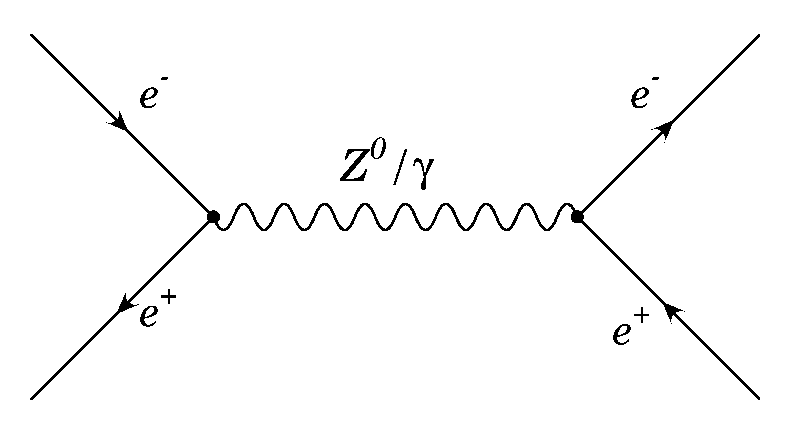
\includegraphics[width=\textwidth]{bhabha-s}
    \caption{$s$-channel Bhaba scattering}
\end{subfigure}
%\hfill
\begin{subfigure}{0.4\textwidth}
    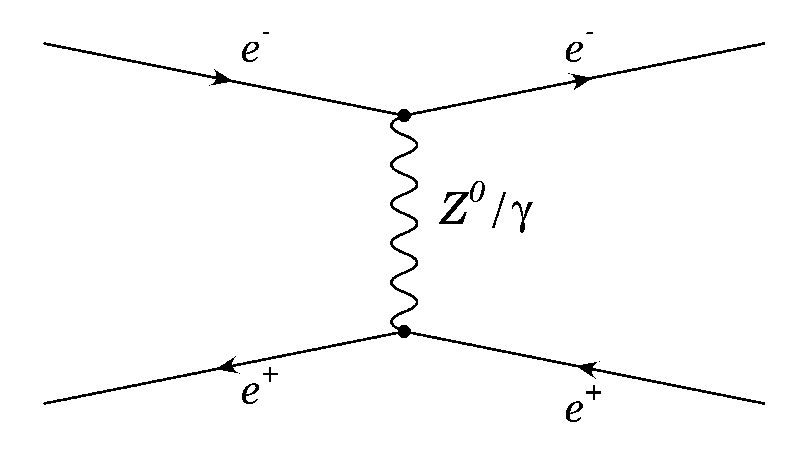
\includegraphics[width=\textwidth]{bhabha-t}
    \caption{$t$-channel Bhaba scattering}
\end{subfigure}
%\hfill
\begin{subfigure}{0.4\textwidth}
\centering
    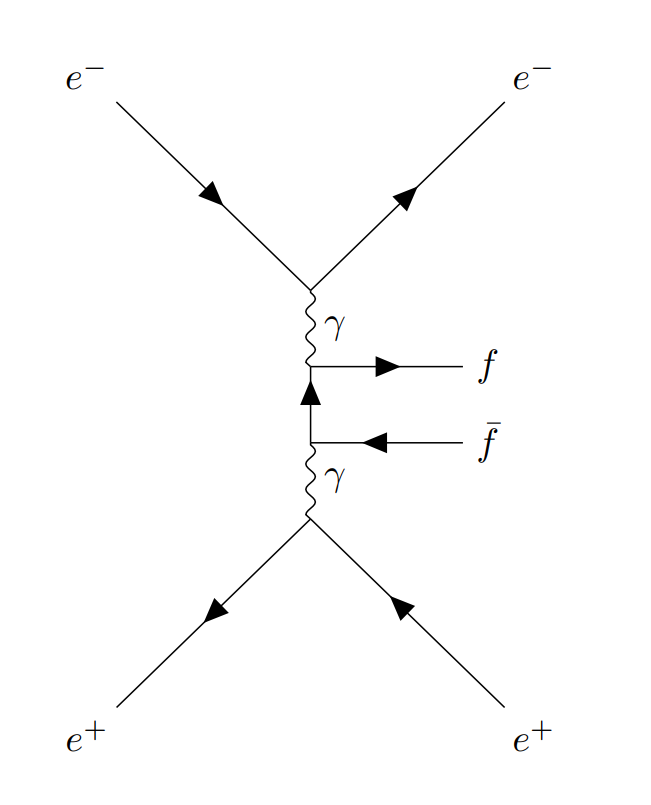
\includegraphics[width=0.9\textwidth]{twophoton}
    \caption{Two photon process}
\end{subfigure}
%\hfill
%\vspace{5em}
\begin{subfigure}{0.4\textwidth}
\centering
    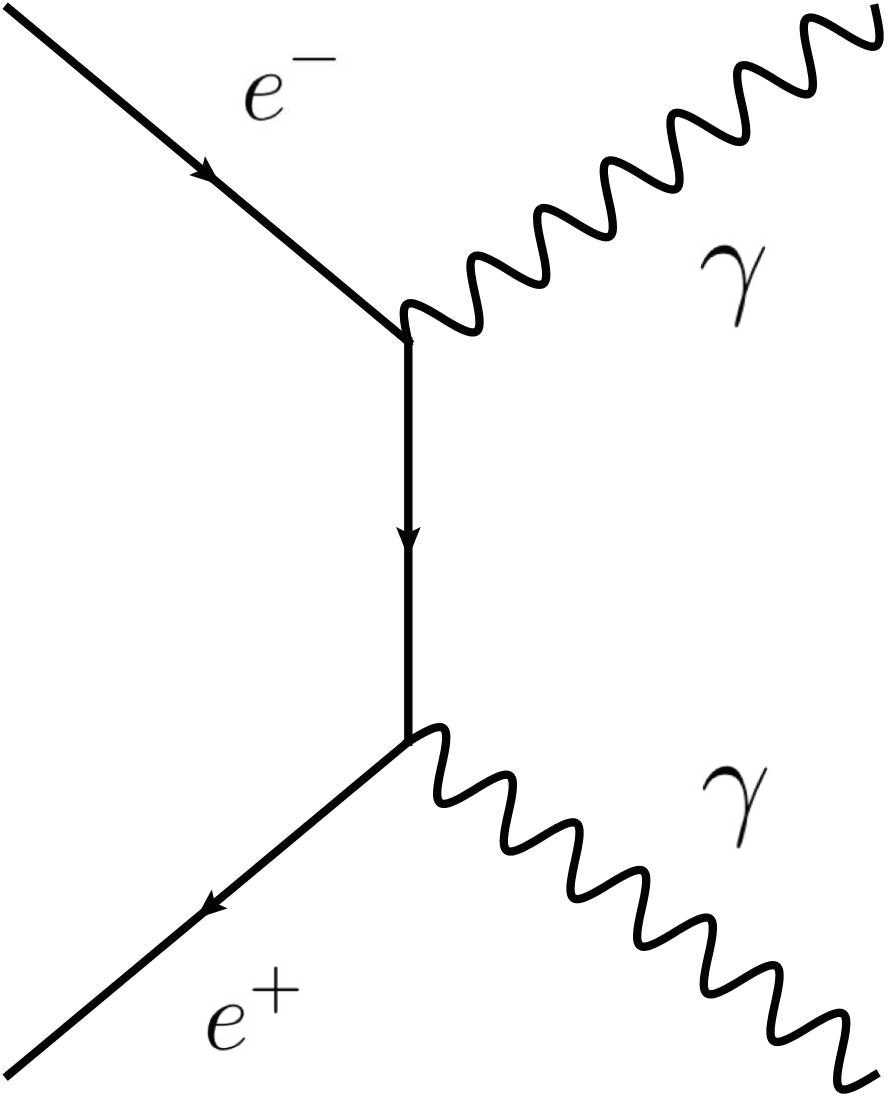
\includegraphics[width=0.7\textwidth]{eeyy}
    \vspace{2em}
    \caption{Production of two photons from $e^{+}e^{-}$ pair}
\end{subfigure}
%\hfill 
\begin{subfigure}{0.45\textwidth}
    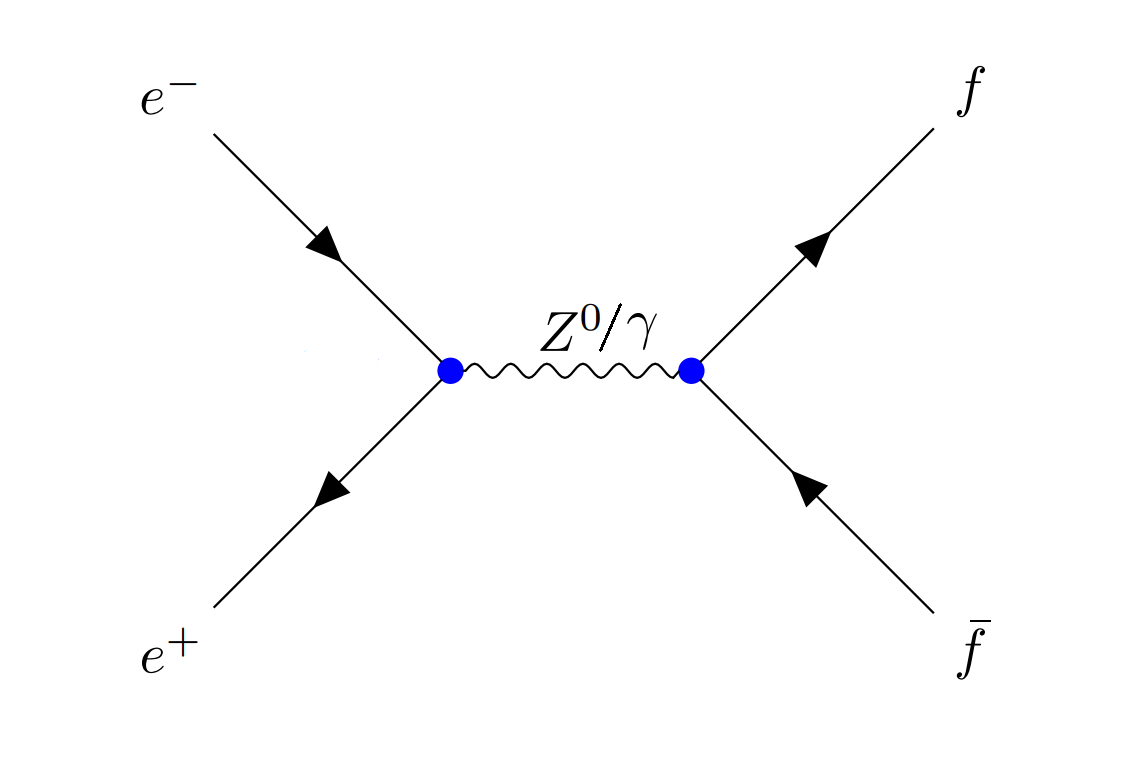
\includegraphics[width=\textwidth]{anihillation}
    \caption{Electron-positron annihilation to $f\bar{f}$}
\end{subfigure}
%\hfill      
\caption[Examples of $e^{+}e^{-}$ interactions]{Examples of $e^{+}e^{-}$ interactions \cite{UB,Janot:2705419,qmdiaries}}
\label{fig:eeint}
\end{figure}

In case of the lowest order $e^{+}e^{-}\rightarrow f \bar{f}$ process, in general, there are contributions to cross section from pure $Z^{0}$, pure $\gamma$ as well as from $\gamma - Z^{0}$ interference terms. However, near center of mass energies close to the $Z^{0}$ resonance, the major contribution to the total cross section is from the pure $Z^{0}$ term.

Additionally, it is easy to see that for the particular case of $e^{+}e^{-}\rightarrow e^{+}e^{-}$ scattering (Bhaba scattering), there is a t-channel contribution in addition to the s-channel component. The cross sections of both these processes have have different angular dependencies \cite{UB}
\begin{align}
\left(\dfrac{d\sigma}{d\Omega}\right)_{s}&\propto (1+\cos^{2}\theta)\\
\left(\dfrac{d\sigma}{d\Omega}\right)_{t}&\propto (1-\cos\theta)^{-2}
\end{align}
This means that while the $s$ channel cross section has a major contribution at large angles (or small values of $\cos\theta$), the $t$-channel contribution increases asymptotically at small angles (or large values of $\cos\theta$). As shall be seen later on, removing the t-channel contribution is an essential step, since we are only concerned with finding the inherent forward-backward asymmetry associated with the $s$-channel processes.

\subsection{Forward-Backward Asymmetry}
\label{FBasymm}
When we consider the $s$-channel processes $e^{+}e^{-}\rightarrow f\bar{f}$, as discussed before, if the process is mediated purely by photons ($\gamma$) then the differential cross section follows the $(1+\cos^{2}\theta)$ dependence and it shows a symmetric dependence on the scattering angle $\theta$. However, for the same process mediated by $Z^{0}$ bosons we find that there is an additional term contributing to the asymmetry:
\begin{equation}
\left(\dfrac{d\sigma}{d\Omega}\right)_{s\ (Z^{0})}\propto a(1+\cos^{2}\theta) + 2b\cos\theta
\end{equation}

From theory of electroweak interactions, this asymmetry (between the number of fermions produced in the forward direction, $\theta>\pi /2$ and the backward direction, $\theta<\pi /2$) can be understood to be arising from the fact that the $Z^{0}$ does not couple equally to right handed and left handed fermions. This becomes more clear by looking at the form of the asymmetry term:
\begin{equation}
b=\left[\left(g_{L}^{e}\right)^{2}-\left(g_{R}^{e}\right)^{2}\right]\left[\left(g_{L}^{f}\right)^{2}-\left(g_{R}^{f}\right)^{2}\right]
\end{equation}
where $g_{L}^{f}$ and $g_{R}^{f}$ signify the coupling of $Z^{0}$ to left handed and right handed fermions respectively. It can be clearly seen that in case the these two couplings had been equal, the asymmetry term would have gone to zero \cite{thomson_2013}.

The forward backward asymmetry factor is given as the ratio:
\begin{equation}
\mathcal{A}_{fb}=\dfrac{\sigma_{F}-\sigma_{B}}{\sigma_{F}-\sigma_{B}}=\dfrac{3b}{4a}
\end{equation}
where $\sigma_{F}$ and $\sigma_{B}$ are the cross sections in forward and backward directions respectively.

It is found that at the resonance of $Z^{0}$ boson, $\mathcal{A}_{fb}$ simplifies to \cite{UB}:
\begin{equation}
\label{eqn:Weinbergangle}
\mathcal{A}_{fb}^{f}\approx 3\left(\dfrac{g_{V}^{f}}{g_{A}^{f}}\right)=1-4\sin^{2}\theta_{W} 
\end{equation}
Thus from the calculation of the forward-backward asymmetry, the ratio of $g_{V}^{f}$ (vector coupling strength between $Z^{0}$ and fermions) to $g_{A}^{f}$ (axial vector coupling strength between $Z^{0}$ and fermions) can be found, which in turn gives us the Weinberg (weak mixing) angle $\theta_{W}$.
\subsection{Background Processes: Radiative Corrections}
In order to test out the predictions of the Standard Model at a very high level of precision, higher order background processes need to be accounted for and as such the corrections made due to these processes are called 'radiative corrections'. The following are some of these processes that need to be accounted for \cite{Zedometry}:
\begin{itemize}
\item \textbf{Initial state radiation (ISR):} The radiation of photons in the initial state lead to decrease in the centre of mass energy and thus affect the $Z^{0}$ resonance peak parameters. This leads to a peak height reduction by upto 25 \%, shift of peak to higher energy and increase in full width at half maximum (FWHM). 
\item \textbf{Final state radiation (FSR):} When photons or gluons are radiated in the final state, it is found that partial widths increase by the corresponding factors:
\begin{equation}
\Delta_{QED}=1+\dfrac{3}{4}\dfrac{Q_{f}^{2}\alpha(m_{Z}^{2})}{\pi}\ ;\ \Delta_{QCD}\approx 1+\dfrac{\alpha_{s}(m_{Z}^{2})}{\pi}
\end{equation}
\item \textbf{QED vacuum polarization:} The production of $e^{+}e^{-}$ pairs from vacuum makes the QED coupling constant scale dependent: 
\begin{equation}
\alpha(0)\rightarrow \alpha(s)=\dfrac{\alpha{0}}{1-\Delta \alpha(s)}
\end{equation}
It has been shown that the imaginary part of $\Delta \alpha(s)$ has an influence on the $\gamma / Z^{0}$ interference term.
\item \textbf{Electroweak corrections:} Further contributions also arise from virtual processes such as higher order loops in $Z^{0}$ propagator and vertex corrections.


Some instances of these radiative corrections are shown in Figure \ref{fig:backfig}
\end{itemize}

\begin{figure}[H]
\centering
\begin{subfigure}{0.45\textwidth}
    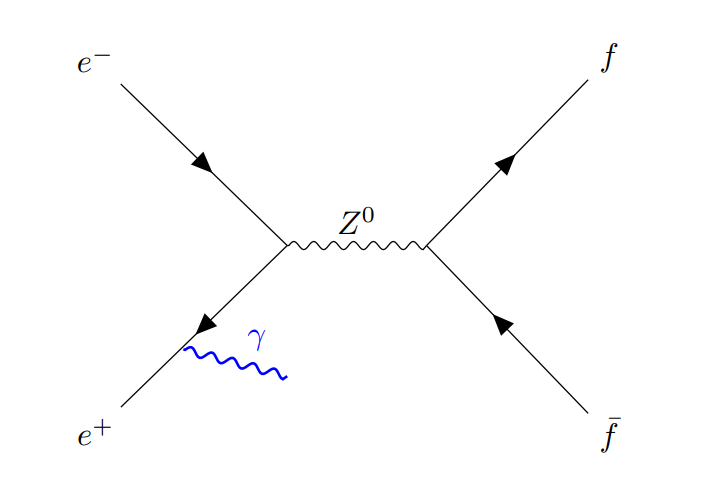
\includegraphics[width=\textwidth]{background1}
    \caption{Initial state radiation (ISR)}
\end{subfigure}
%\hfill
\begin{subfigure}{0.45\textwidth}
    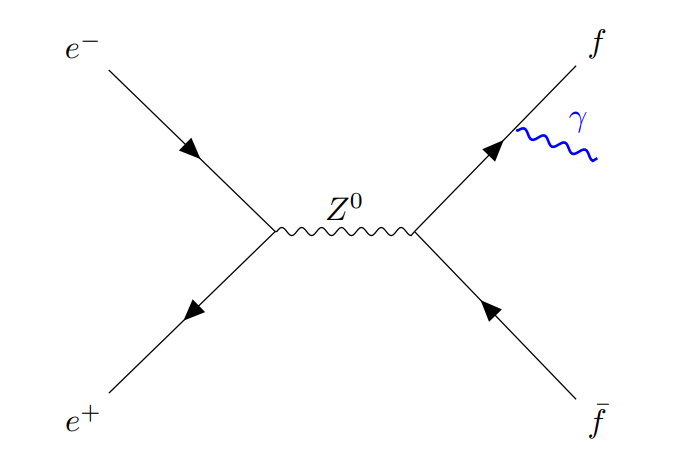
\includegraphics[width=\textwidth]{background2}
    \caption{Final state radiation (FSR)}
\end{subfigure}
%\hfill
\begin{subfigure}{0.45\textwidth}
    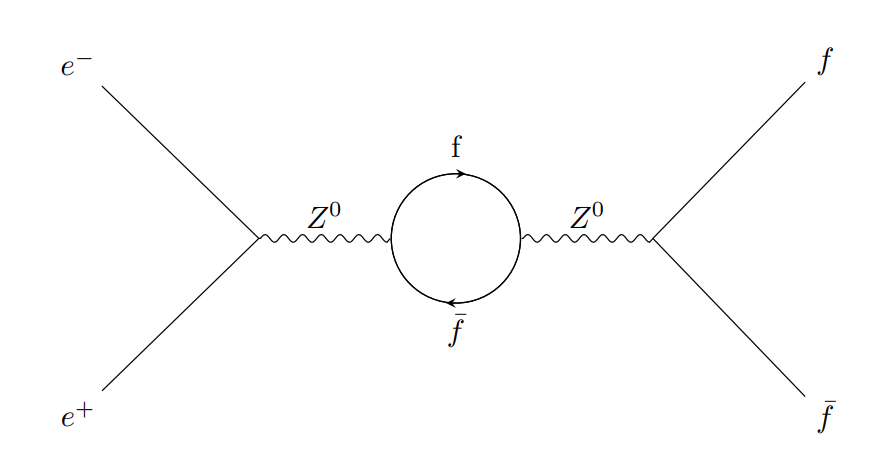
\includegraphics[width=\textwidth]{background3}
    \caption{$Z^{0}$ propagator correction}
\end{subfigure}
%\hfill
\begin{subfigure}{0.45\textwidth}
    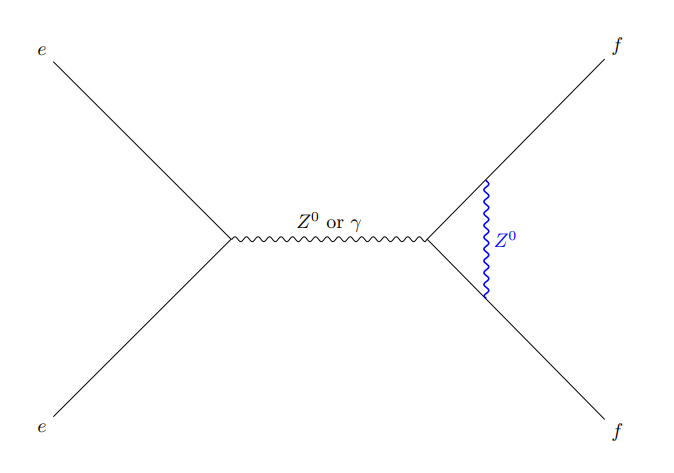
\includegraphics[width=\textwidth]{background4}
    \caption{$Z^{0}$ vertex correction}
\end{subfigure}       
\caption[Examples of radiative corrections]{Examples of radiative corrections \cite{UB}}
\label{fig:backfig}
\end{figure}

\subsection{Mass and Width of the $Z^{0}$ Boson}
From the theory of electroweak interactions, it is known that the contribution the $Z^{0}$ boson exchange propagator to the matrix element (in s-channel processes) can be given by:
\begin{equation}
\mathcal{M}_{Z^{0}}\propto \dfrac{g_{Z^{0}}^{2}}{q^{2}-m_{Z^{0}}^{2}}=\dfrac{g_{Z^{0}}^{2}}{s-m_{Z^{0}}^{2}}
\end{equation}
While one can see from this dependence that at low energies ($\sqrt \ll m_{Z^{0}}$), QED processes dominate and at high energies ($\sqrt{s}\gg m_{Z^{0}}$), the $Z^{0}$ exchange also becomes important; we see that around the $Z^{0}$ resonance ($\sqrt{s}\sim  m_{Z^{0}}$), the propagator diverges. In order to correct for this, it is necessary to introduce a modification in the propagator for a decaying state. When an unstable particle has a decay rate $\Gamma$, its wavefunction gets modified to:
\begin{equation}
\psi\propto e^{-imt}\rightarrow e^{-imt}
\end{equation} 
which is equivalent to introducing an additional imaginary term in the mass:
\begin{equation}
m\rightarrow m-i\dfrac{\Gamma}{2}
\end{equation}
Accordingly, the $Z^{0}$ propagator then changes to:
\begin{equation}
\dfrac{1}{s-m_{Z^{0}}^{2}}\rightarrow \dfrac{1}{s-m_{Z^{0}}^{2}} 
\end{equation}
On simplifying this result, taking the spin averaged matrix element and inserting the appropriate pre-factors, the complete form of the cross section in the process $e^{+}e^{-}\rightarrow Z^{0}\rightarrow f\bar{f}$ is given by:
\begin{equation}
    \sigma_f (s) = \frac{12\pi}{M_Z^2} \frac{s \Gamma_e \Gamma_f}{(s-M_Z^2)^2 + \left(\frac{s\Gamma_Z}{M_Z}\right)^2} (\hbar^2 c^2),
\end{equation} 
The probability distribution that characterizes the dependence of this cross section of the centre of mass energy is called the Breit-Wigner distribution. This distribution is shown in Figure \ref{fig:BWdist}.

\begin{figure}[H]
\centering
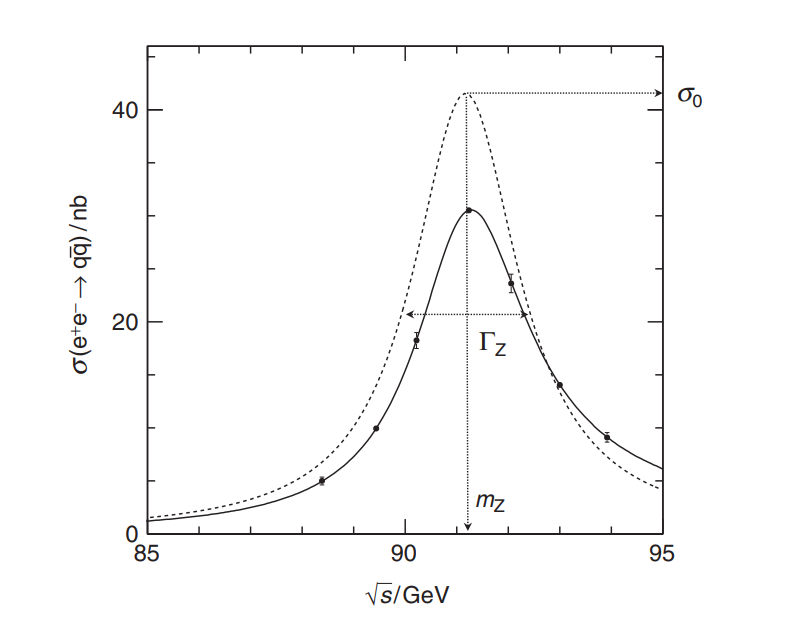
\includegraphics[width=0.6\textwidth]{BWdist}
\caption[Breit Wigner distribution of the cross section for $e^{+}e^{-}\rightarrow q\bar{q}$ process]{The Breit Wigner distribution of the cross section for $e^{+}e^{-}\rightarrow q\bar{q}$ process at centre of mass energies around the $Z^{0}$ resonance (the dashed and solid curves are the distribution after and before corrections for initial state radiation). \cite{thomson_2013}}
\label{fig:BWdist}
\end{figure}
As can be seen from the figure, at the $Z^{0}$ resonance, the physical parameters of the $Z^{0}$ can easily be extracted. For example, the mass of the $Z^{0}$ would simply be the value on the $x$ axis where this peak occurs, its decay width can be found from the full width at half maximum (FWHM) of the curve, and reading off the $y$ value at the resonance peak gives us the resonant cross section. This will in fact be one of the important tasks of the present experiment.

\section{LEP Experiment and the OPAL Detector}
The Large Electron Positron Collider (LEP) was built at CERN, with one of its major goals being making high precision measurements of the parameters of the $Z^{0}$ boson, such as its mass, decay width and angular distributions of final state particles produced from $Z^{0}$ decays. As such, for most of its period of operation from 1989 to 1995, it produced $e^{+}e^{-}$ collisions at centre of mass energies very close to the $Z^{0}$ resonance and about 17 million $e^{+}e^{-}\rightarrow Z^{0}$ events were recorded in this time frame \cite{thomson_2013}. It was built in such a manner that the electron-positron collisions took place at four different points in the circular collider, and hence four such detectors were used in this experiment: ALEPH (Apparatus for LEP PHysics), DELPHI (DEtector with Lepton, Photon and Hadron Identification), L3 (Third LEP experiment) and OPAL (Omni-Purpose Apparatus for LEP). 

The components of the OPAL detector shall be described in further detail in this Section, since this experiment focuses on analysis of data collected by the OPAL.

\subsection{The OPAL Detector}
\begin{figure}[H]
\centering
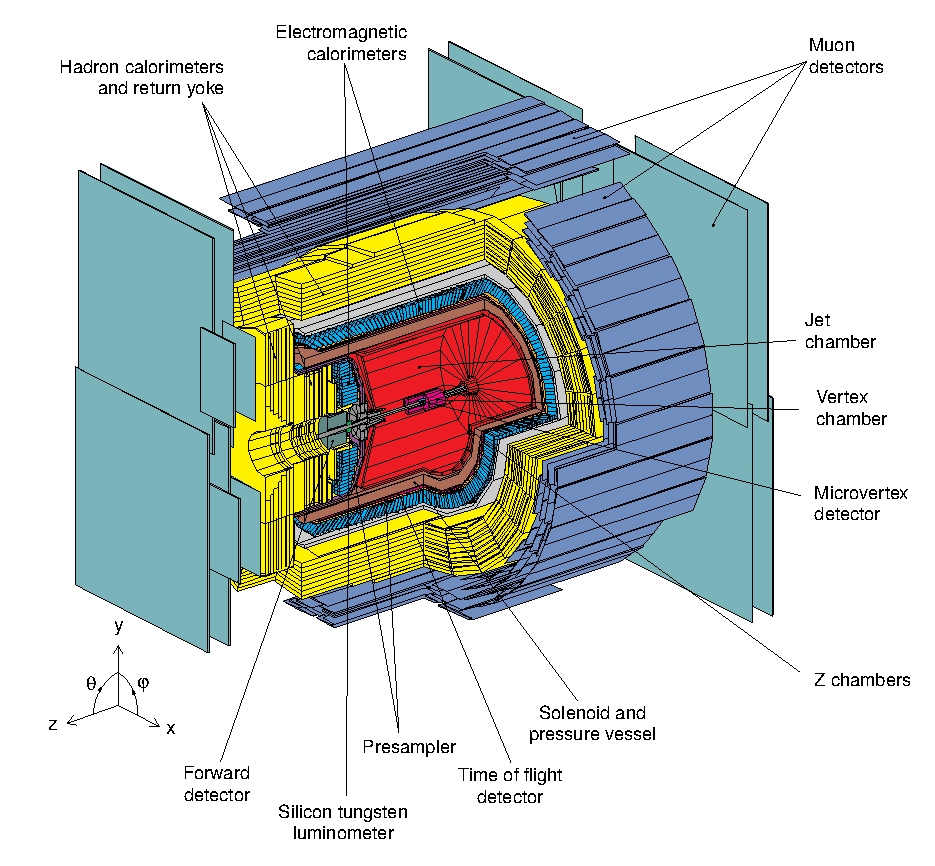
\includegraphics[width=0.69\textwidth]{OPAL1}
\caption[The OPAL Detector and its various components]{The OPAL Detector and its various components \cite{OPAL}}
\label{fig:OPAL}
\end{figure}

For analysis of events arising from this detector, a right handed coordinate system is followed. The origin is fixed at the point where $e^{+}e^{-}$ collisions take place, the $x$ axis points horizontally in the direction of the center of the LEP, while the z axis is defined to lie along along the beam path and the y axis is then just perpendicular to the $x-y$ plane as usual. $\theta$, the polar angle is the angle between the $y$ and $z$ axes and the azimuthal angle $\phi$ is the counterclockwise angle between the $x$ and $y$ directions. The OPAL detector and this coordinate system is displayed in Figure \ref{fig:OPAL}.

Starting from the origin, as the $e^{+}e^{-}$ collision products fly outwards, various detector components are encountered which serve to detect the type and various characteristics of the final state particles. These primary detector components are discussed here in brief \cite{UB,1991275}:
\begin{itemize}
\item \textbf{Vertex detector:} This is a type of drift detector that surrounds the central beam pipe and plays a key role in locating vertices of short-lived decay products and also helps in improving the momentum resolution. It has dimensions of 1 m in length and measures 470 mm across (diameter), layered with 36 axial cells that measure positions in the $r-\phi$ plane.  
\item \textbf{Jet chamber:} This is again a cylindrical drift chamber with a good spatial and track resolution, designed in a manner so as to efficiently record events associated with jets. Inside this chamber, there are 24 sectors, each of which contains 159 sensing wires, arranged parallel to the beam axis. Beside the anode wires, there are alternating potential wires and cathode wires positioned in between the potential and anode wires. The coordinates of the decay particles are obtained from parameters such as the positions of the wires and the drift time. Moreover, the signals from these wires determine the energy loss $dE/dx$ of charged particles in this region.
\item \textbf{$\mathbf{z}$ chambers:} As the name suggests, the $z$ chambers serve the purpose of locating the $z$ coordinates of decay particles when they leave the jet chamber. As such they are helpful in improving the resolutions of the polar angle and invariant mass distributions of charged particles. Consisting of 24 drift chambers, subdivided into 8 cells each, a high $z$ resolution of 100-200 $\mu$m is achieved by these chambers.
\item \textbf{Solenoid:} The solenoid surrounds the detectors discussed so far (categorized under central detector) and generates a uniform magnetic field of 0.435 T along the beam direction. The magnetic field makes the charged particles follow a helical path in the central detectors and therefore is essential to measure their momenta. 
\item \textbf{Time of flight (TOF) system:} The role of the TOF system is to generate signals (light from a total of 160 scintillation chambers) that trigger the detector and to identify charged particles in the range of 0.6 to 2.5 GeV. Further it is useful in rejecting cosmic rays.
\item \textbf{Electromagnetic calorimeter (ECAL):} This detector is made up of 9440 blocks of lead glass. The geometry of this detector is in the form of a barrel around the jet chamber with two endcaps, covering a total of 98 \% of the solid angle. Particles such as photons, electrons and positrons deposit all of their energy in the ECAL either through Bremsstrahlung ($e^{+}$ or $e^{-}$ emitting a photon) or by pair production (a photon giving rise to an $e^{+}e^{-}$ pair). Hadrons on the other hand, do deposit some of their energy here (in the form of electromagnetic showers), but mostly don't come to a stop in the ECAL. The reason for choosing lead glass for the ECAL is that the material provides an excellent resolution of:
\begin{equation}
\dfrac{\sigma_{E}}{E}\approx \dfrac{5 \%}{\sqrt{E}}
\end{equation}
\item \textbf{Hadron calorimeter (HCAL):} This detector has a similar geometry to that of that of ECAL and serves to detect mesons and baryons. The hadrons however do not lose all their energy through ionisation but also undergo strong interaction with the nuclei that they encounter on their way. As such there can be numerous decay products in the associated hadronic showers. Furthermore, since the decay products travel significant distances between any two nuclear interactions, the HCAL occupies much more volume of the detector than ECAL and is made up of absorber material with a high density (iron slabs in this case). Because of the uncertainties in determining the amount of energy lost electromagnetically and in the energy loss in nuclear interactions, the energy resolution for the HCAL is much than that of the ECAL:
\begin{equation}
\dfrac{\sigma_{E}}{E}\approx \dfrac{120 \%}{\sqrt{E}}
\end{equation} 
\item \textbf{Muon detector:} Outside the HCAL, lie four layers of muon detectors. The muon detector provides a coverage of almost the entire solid angle of 4$\pi$ and has a barrel region and two endcap regions, similar to the ECAL and HCAL. The detection probability of muons having an energy greater than 3 GeV in this region is quite close to 100 \% because almost all of the other decay products have either been absorbed in the ECAL or in the HCAL.
\end{itemize}
